%#!pdfpLaTeX
%
% 北村研究室用卒論予稿のTeXテンプレートファイル
% 本ファイルは非公式であり,下記で公開されているワードのテンプレートが公式である.
% https://www.kagawa-nct.ac.jp/EE/local/index.html (学内限定アクセス)
%
% 2020年1月18日 北村大地作成
%

\documentclass[a4j]{jsarticle}
\usepackage{nitkagawaproc5ec} % 予稿テンプレートクラスファイル
\usepackage{amsmath,amssymb} % 数式環境
\usepackage{bm} % 数式の太字斜体
\usepackage[dvipdfmx]{color}
\usepackage[dvipdfmx]{graphicx}
\usepackage{flushend} % 2段組みの最終ページの高さを揃える

\renewcommand{\baselinestretch}{0.8} % 行間設定(標準は0.8)
\newcommand{\red}[1]{\textcolor{black}{#1}}
\newcommand{\blue}[1]{\textcolor{blue}{\Sl{}}}

%%%%%%%%%%%%%%%%%%%%%%%%%%% 論文情報 %%%%%%%%%%%%%%%%%%%%%%%%%%%

%%%%% タイトル %%%%%
\title{深層パーミュテーション解決法の基礎的検討}
\etitle{Basic study for deep permutation solver.}

%%%%% 著者 %%%%%
\author{蓮池 郁也}
\eauthor{Fumiya Hasuike}


%----- 図表題が英語の場合は次の2行を有効化 -----%
\renewcommand{\figurename}{Fig.~} 
\renewcommand{\tablename}{Table~}
%--------------------------------------------%

\begin{document}
\maketitle% タイトル生成

%----- ハイフン付きページ番号を表示する場合は次3行を有効化 -----%
%\setcounter{page}{1} % 開始ページ番号(3にすると3ページと4ページの2枚になる)
%\pagestyle{hyphenpage}
%\thispagestyle{hyphenpage}
%---------------------------------------------------------%

%----- ハイフン無しページ番号を表示する場合は次3行を有効化 -----%
%\setcounter{page}{1} % 開始ページ番号(3にすると3ページと4ページの2枚になる)
%\thispagestyle{plain}
%\pagestyle{plain}
%---------------------------------------------------------%

%----- ページ番号を削除する場合は次2行を有効化 -----%
\thispagestyle{empty}
\pagestyle{empty}
%-----------------------------------------------%

%%%%%%%%%%%%%%%%%%%%%%%%%%% 本文 %%%%%%%%%%%%%%%%%%%%%%%%%%%
%----------------------------------------------
\section{はじめに}
%----------------------------------------------
音源位置やマイクロフォン位置等が未知の条件で音源分離を達成する技術はブラインド音源分離(BSS)と呼ばれる.
観測信号のチャネル数(マイクロフォン数)と混合されている音源数が等しい条件下では,観測信号を時間周波数領域に変換し周波数毎に独立成分分析(ICA)\cite{ICA}を適用する時間周波数領域ICA(FDICA)\cite{FDICA}が提案されている.
ここで,ICAは一般に推定分離信号の順番が不定であり,FDICAは周波数毎に独立なICAによるBSSを行うため,分離信号の順番が周波数毎にばらばらになってしまう問題が生じる.
この問題は一般に「パーミュテーション問題」と呼ばれている.

本稿では,前述の問題を解決するために深層学習(DNN)に基づくパーミュテーション解決法を検討する.
また,本論文で提案する深層パーミュテーション解決法を人工データと実際の音声及び音楽信号に適用し,DNNに基づくパーミュテーション問題解決の可能性について調査する.

%----------------------------------------------
\section{従来手法}
%----------------------------------------------

%----------------------------------------------
\subsection{FDICAとパーミュテーション問題}
%----------------------------------------------
FDICAは音源間の統計的独立性のみに基づいて分離行列を推定するため,分離音源のスケール及び順番に関して推定することができない.
従って,FDICAの推定分離行列を$\hat{\bm{W}}_i$とすると,次式のような不定性が残る.
\begin{align}
	\hat{\bm{W}}_{i} &= \bm{D}_{i}\bm{P}_{i}  \bm{W}_{i} \label{eq:w_fdica}
\end{align}
ここで,$i=1,2,\cdots,I$は周波数ビンのインデクス,$\bm{W}_{i}$は分離行列,$\bm{P}_i \in \{0, 1\}^{N \times N}$は分離行列$\bm{W}_{i}$の行ベクトル$\bm{w}_{in}$の順番を入れ変えうるパーミュテーション行列(置換行列),
$\bm{D}_i \in \mathbb{R}^{N \times N}$は,$\bm{w}_{in}$のスケールを変化させる可能性のある対角行列を表す.

従って,FDICAで推定される分離信号
\begin{align}
\bm{y}_{ij} &= \hat{\bm{W}}_i\bm{x}_{ij} \\
&=\left[ y_{ij1},y_{ij2}, \cdots, y_{ijn}, \cdots, y_{ijN} \right]^\mathrm{T}~\in \mathbb{C}^{N} \label{eq:sepSig}
\end{align}
は,推定音源の順番やスケールが周波数毎にばらばらになっている状態である.その概念図をFig.~\ref{fig:permu}に示す.
ここで,$\bm{y}_{ij}$は分離信号,$\bm{x}_{ij}$は観測信号,$j=1,2,\cdots,J$は時間フレーム数を表す.
FDICAで得られる(パーミュテーション問題が生じている状態の)推定信号$\bm{y}_{ij}$の$n$番目のスペクトログラムを$\bm{Y}_n \in \mathbb{C}^{I \times J}$と定義する.
このうち,$\bm{D}_i$によって生じるスケールの任意性は,プロジェクションバック法\cite{Matsuoka2001_PB}で解析的に復元可能である.
一方で,$\bm{P}_i$によって生じる分離信号の順番の任意性(パーミュテーション)を$I$個の全周波数ビンに関して復元することは,組み合わせ爆発が生じるため容易ではない.
このパーミュテーション問題を解決する処理は次式で表される.
\begin{align}
\bm{z}_{ij} &= \bm{P}_{i}^{-1}\bm{D}_{i}^{-1}\bm{y}_{ij} \label{eq:z}
\end{align}
従って,パーミュテーション問題の解決とは,全周波数ビンにわたって$\bm{P}_{i}^{-1}$を求める問題として解釈できる.

%%%%%%%%%%%%%%%%%%%%%%%%%%%%
\begin{figure}[t]
  \begin{center}
      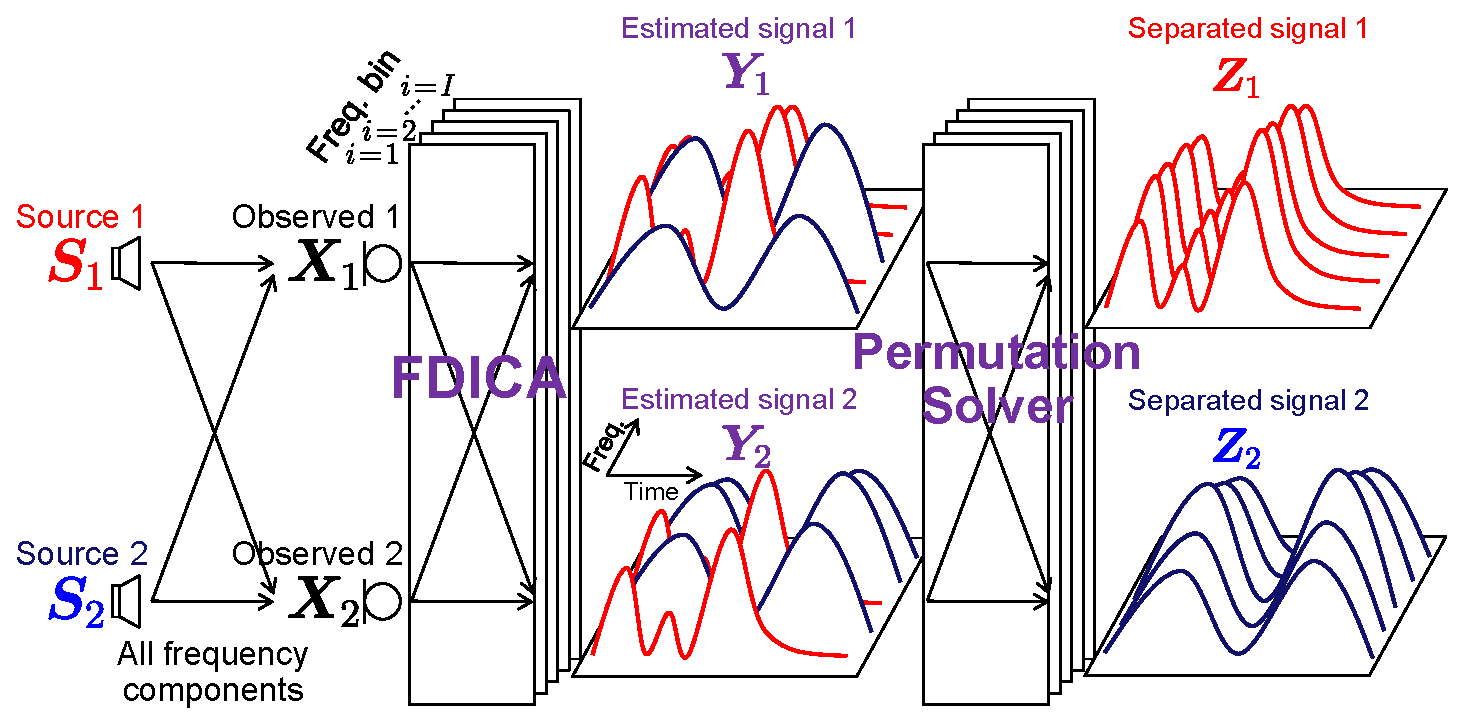
\includegraphics[width=0.95\columnwidth]{figures/permutation_image.eps}
  \end{center}
  \vspace{-8pt}
\caption{Permutation problem in FDICA, where $N=M=2$.}
\label{fig:permu}
\end{figure}
%%%%%%%%%%%%%%%%%%%%%%%%%%%%

%----------------------------------------------
\section{提案手法}
%----------------------------------------------

%----------------------------------------------
\subsection{DNNの入出力}
%----------------------------------------------
\red{同一音源に属する成分の相関を強調するため,推定信号$(\bm{Y}_1, \bm{Y}_2)$のパワースペクトラム$(|\bm{Y}_1|^{.2}, |\bm{Y}_2|^{.2})$の比率に変換する正規化\cite{Permutation_solverBSS}を施す.}
推定信号の正規化振幅スペクトログラム$(\overline{\bm{Y}}_1, \overline{\bm{Y}}_2)$から,時間フレーム$j$を中心とする局所時間振幅スペクトログラムを抽出し,一次元に整形(ベクトル化)したものをDNNの入力とした.
DNNによる出力は次式で表される.
\begin{align}
    \red{\hat{\bm{l}}_j = \mathrm{DNN}(\bm{d}_j) \in [ 0, 1 ]^{2I}}
\end{align}
ここで,$\hat{\bm{l}}_j = [ \hat{l}_{11j}, \hat{l}_{21j}, \cdots, \hat{l}_{I1j}, \hat{l}_{12j}, \hat{l}_{22j}, \cdots, \hat{l}_{I2j} ]^\mathrm{T}$は出力である予測ベクトルを表す.
またDNNの出力にはsoftmax関数を用い,確率値とした.
2つのパーミュテーション問題が生じている入力信号$(\check{\bm{Y}}_{j1}, \check{\bm{Y}}_{j2})$の各周波数成分のそれぞれが
「1番目の音源の成分である確率$l_{i1}$」と「2番目の音源の成分である確率$l_{i2}$」を入力ベクトルから予測したものと定義し,提案手法ではこの定義に基づいて正確な予測ができるDNNを学習する.

%----------------------------------------------
\subsection{DNNの構造}
%----------------------------------------------
%%%%%%%%%%%%%%%%%%%%%%%%%%%%
\begin{figure}[t]
  \begin{center}
      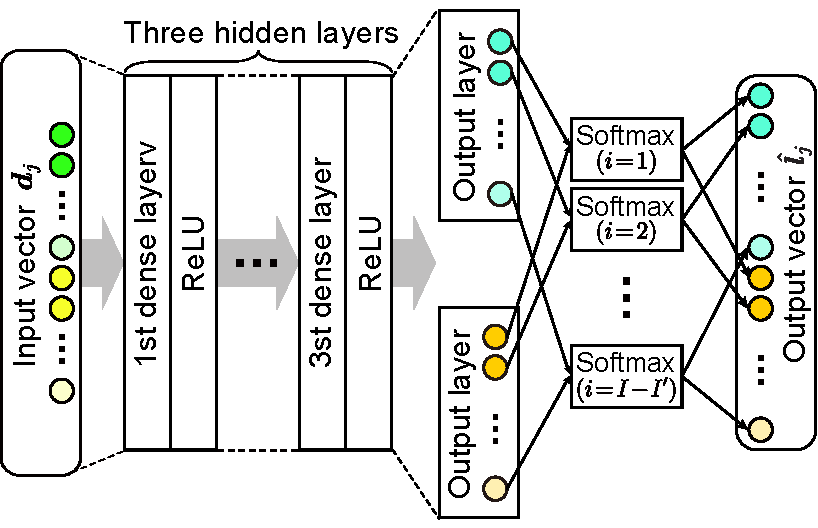
\includegraphics[width=0.8\columnwidth]{figures/architecture_DNN.pdf}
  \end{center}
  \vspace{-8pt}
\caption{DNN architecture.}
\label{fig:Dnnmodel}
\end{figure}
%%%%%%%%%%%%%%%%%%%%%%%%%%%%
Fig.~\ref{fig:Dnnmodel}に提案深層パーミュテーション解決法で用いるDNNの構造を示す.
DNNは入力層,隠れ層3層,及び出力層の計5層の全結合層からなるMLPとなっている.

%----------------------------------------------
\subsection{DNN学習時の損失関数}
%----------------------------------------------
損失関数には平均二乗誤差(MSE)を用いる.
具体的には.DNNの出力である予測ベクトルに従って,推定信号$(\bm{Y}_1, \bm{Y}_2)$を並び替えを行い正解の分離信号の間で平均二乗誤差(MSE)を使用する.


本文中に数式を挿入する場合は,次に示すように中央寄せすると良い.
\begin{align}
  \nonumber  a^2 + b^2 = c^2
\end{align}
複数行の数式を挿入する場合は,次のように等号記号で左右位置をそろえる.
\begin{align}
  \nonumber  a^2 + b^2 &= c^2 \\
  \nonumber d^2 &= e^2 + f^2 \\
  \nonumber A + B + C &= E + F + G
\end{align}
横に長すぎる数式は改行を設けることで対処できる.
但し,可能な限り左辺と右辺の左右位置は重ならないようにすることが望ましい.
\begin{align}
  \nonumber  A &= B + C + D + E + F + G + H + I + J + K \\
  \nonumber &\phantom= + L + M + N + O + P
\end{align}
縦に幅を取る数式を挿入すると次のようになる.
\begin{align}
  \nonumber  f(x) = a_0 + \sum_{n=1}^{\infty} \left( a_n \cos \frac{ n\pi x }{ L } + b_n\sin \frac{ n\pi x }{ L } \right)
\end{align}
なお,数式中に登場した変数等は全て登場直後に説明されなければならない.
その一例を次式に示す.
\begin{align}
  \nonumber  x = \frac{ -b \pm \sqrt{ b^2 -4ac } }{ 2a }
\end{align}
ここで,$a$は2乗項の係数,$b$は1乗項の係数,$c$は定数項をそれぞれ示す.
本文全体で未定義の変数が残っていないか十分注意すること.

一度登場した数式を後の本文で引用する場合は,次式のように数式の右側に式番号を付与する.
\begin{align}
  A = \pi r^2 \label{eq:radius}
\end{align}
式番号は括弧書きの数字とし,登場する順番に番号を付与する.
式番号を用いて数式を引用する場合は「式(\ref{eq:radius})」又は「(\ref{eq:radius})式」と記述する.
どちらを用いても良いが,表記は本文全体で統一されている必要がある.

文中(インライン)に数式を挿入することもできる.
例えば,$f(x) = 1/2 \sin(\alpha + \beta)$のように記述できる.
ただし,縦に幅を取る数式はインラインで記述することは避けるべきである.
また分数も,インラインで表記する場合は$V = 4/3\pi r^3$のようにスラッシュ記号を用いて縦の幅を節約する工夫をする.

%----------------------------------------------
\subsection{参考文献の引用の挿入方法}
%----------------------------------------------

本文の適切な箇所で参考文献を引用する場合は,このように記述する\cite{sample1}.
この引用番号を表す記号は,予稿の末尾に記載されている参考文献リストと対応している\cite{sample2}.
但し,登場する順に番号を付与する.
なお,参考文献として不適切な文書を引用してはいけない.
例えば,信憑性が疑われるインターネット上の記事(ブログ,ウィキペディア,ニュース等)や学術的でない雑誌等は引用を避けるべきである.
厳正な査読を経て掲載された原著論文及び国際会議論文が最も適切であるが,確立された技術を網羅した教科書等を引用する場合もある.
その他,他者の学位論文(修士論文,博士論文等)を引用することもあるが,これらの多くは信憑性が疑われるものも多々あるので十分注意する.

%----------------------------------------------
\section{まとめ}
%----------------------------------------------

以上の方法で作成すると,正しい体裁の技術文書を作成することができる.
より読みやすく正しい技術文書を作成するためには,詳細を解説した参考書等を参考にすること.
また,予稿完成後も複数人で念入りにチェックを繰り返し,誤字や脱字,不適切な記述,数式の誤り等が無いように十分注意すること.

%----------------------------------------------
\section{注意事項}
%----------------------------------------------

本テンプレートは元々Wordでのみしか配布されていなかった卒業研究発表会予稿のテンプレートを,北村大地がLaTeXによる組版で可能な限り忠実に再現したファイルになります.
マージンや余白などには細心の注意を払いましたが,ボールドフォントの違い等の細かい点は組版ソフトの違いが存在する以上生じてしまいます.
あくまでも非公式のテンプレートとして自己責任で使用してください.

TeXのコンパイラは恐らく最もスタンダードであるpdfpLaTeXを使用することを想定しています.
他のコンパイラでの動作確認はしておりません.
また,今後の対応の予定もありません.
もう北村は疲れました.


%%%%% 参考文献 %%%%%
\begin{thebibliography}{9}% 10以上の文献数であれば99とする
%参考文献のフォントサイズを小さくしたい場合は下記2行のコメントアウトを解除
%\itemsep 3pt % 項目の間隔微調整用
%\fontsize{8pt}{10pt}\selectfont  % 項目のフォントサイズ微調整用

\bibitem{ICA}
P.~Comon, ``Independent component analysis, a new concept?," {\em Signal Process.}, vol. 36, no. 3, pp. 287--314, 1994.

\bibitem{FDICA}
P.~Smaragdis, ``Blind separation of convolved mixtures in the frequency domain," {\em Neurocomputing}, vol. 22, pp. 21--34, 1998.

\bibitem{Matsuoka2001_PB}
K.~Matsuoka and S.~Nakashima, ``Minimal distortion principle for blind source separation,'' {\em Proc. ICA}, pp. 722--727, 2001.

\bibitem{Permutation_solverBSS}
\red{H. Sawada, S. Araki, and S. Makino, ``Measuring dependence of bin-wise separated signals for permutation alignment in frequency-domain BSS,'' Proc. ISCAS, pp. 3247--3250, 2007.}

\end{thebibliography}

\end{document}